\documentclass[fleqn,10pt]{wlscirep}
\usepackage[utf8]{inputenc}
\usepackage{units}
\usepackage{makecell}
\usepackage{float}
\usepackage[T1]{fontenc}
\title{Sustained changes to urban mobility after COVID-19 amplified socio-economic inequalities in Latin America}



\author[1,2,*,\textsuperscript{\textdagger}]{Carmen Cabrera}
\author[1]{Miguel González-Leonardo}
\author[1,3]{Andrea Nasuto}
\author[2]{Ruth Neville}
\author[1,\textsuperscript{\textdagger}]{Francisco Rowe}
\affil[1]{Geographic Data Science Lab, Department of Geography and Planning, University of Liverpool, Liverpool, UK}
\affil[2]{Centre for Advanced Spatial Analysis, University College London, London, UK}
\affil[3]{Institute for Quantitative Social Science, Harvard University, Cambridge, US}


\affil[*]{Corresponding author: c.cabrera@liverpool.ac.uk}

\affil[ \textsuperscript{\textdagger}]{These authors have contributed equally to this study.}

%\keywords{Keyword1, Keyword2, Keyword3}


\begin{abstract}
Urban mobility is central to economic activity, social inclusion and access to services. COVID-19 caused disruptions to mobility globally, yet its long-term impacts in less developed countries remain poorly understood. Using $>$170 million anonymised and aggregated location records from Meta-Facebook users in Argentina, Chile and Colombia (April 2020–May 2022), we examine changes in overall mobility volume relative to pre-pandemic baselines across socioeconomic and rural–urban gradients. We find the sharpest declines and most persistent reductions below baseline in high-density and affluent areas, while low-density and more deprived communities returned to baseline levels. These differences are explained mainly by the scale of the initial mobility shock rather than by subsequent recovery rates. Our findings reveal how a global shock can entrench disparities in human mobility, with implications for economic resilience, social inclusion and urban planning in unequal nations. Our study underscores the need for proactive policies to prevent long‑lasting inequalities in mobility.

%The COVID-19 pandemic caused unprecedented disruptions to urban mobility patterns. Existing work has overwhelmingly focused on the immediate impacts of COVID-19 on human mobility during 2020, particularly in more developed countries. It showed that COVID-19 restrictions led to unequal effects: greater reductions in mobility in less deprived and high-density areas than in more deprived and less dense communities. However, little is known about the long-term persistence of these unequal impacts beyond 2020, and in less developed countries where socioeconomic disparities are more acute. Using over 100 million anonymised daily records of mobile phone data from Meta-Facebook users from March 2020 to May 2022, we aim to determine the long-term geographic and socioeconomic impact of COVID-19 on mobility patterns in Latin American countries (Argentina, Chile and Colombia). Our findings reveal sustained differences in mobility after the immediate effects of COVID-19 in 2020 extending beyond early 2022. Less deprived and high-density areas continued to display lower mobility levels than more deprived and less dense communities. We also show that the magnitude of the initial mobility reduction largely determined the extent of differences in mobility levels across socioeconomic groups over time. We find a sustained reduction in net mobility flows in core and dense urban areas, suggesting that cities lost attraction power as daily centres of gravity. Our findings suggest that the COVID-19 pandemic has contributed to amplified pre-existing socioeconomic inequalities. Targeted interventions to close the recovery gap need to be directed to support mobility in hard-hit urban centres (e.g. reconfiguring urban public transit), rural areas (reconnecting isolated communities) and assisting more deprived communities (mitigating travel costs). Overall, our research contributes evidence to building more resilient mobility systems that allow returning to daily life more efficiently and equitably after major disaster shocks.

\end{abstract}

\begin{document}

\flushbottom
\maketitle
% * <john.hammersley@gmail.com> 2015-02-09T12:07:31.197Z:
%
%  Click the title above to edit the author information and abstract
%
\thispagestyle{empty}

Cities were epicentres of the COVID-19 pandemic. By November 2020, approximately 95\% of all the reported infections and fatalities had concentrated in a few large cities \cite{Pomeroy2021}. Stringency measures to contain the spread of COVID-19 reshaped the global patterns of urban mobility in the early months of 2020 \cite{nouvellet2021}. Social distancing, lockdowns, and business and school closures forced sharp declines in human mobility, notably in large cities \cite{florida2021}, responding to a need for limited social face-to-face contact and a transition to increased digital interaction. Against this backdrop, media headlines portrayed a gloomy prospect for cities pointing to an ``urban exodus'' with anecdotal evidence showing an intensification in the relative number of people moving from large cities to suburbs and rural locations \cite{paybarah2020new, marsh2020escape}.

Subsequent scientific studies examined these patterns, providing empirical evidence for widespread reductions in the intensity of both short- and long-distance movements from cities \cite{de2022overview}, particularly during the outbreak of the COVID-19 pandemic in the early months of 2020. While the extent of these changes varied widely across cities \cite{hunter2024city, kephart2021effect, fatmi2020, Chin24}, they were consistently documented across many developed and developing countries during the early months of 2020 \cite{nouvellet2021, rowe2023}. This evidence also points to a temporary reallocation of urban space towards active mobility, often reflected in increases in walking and cycling \cite{brooks2021, DavoudiZavareh2025, Delbosc25, An2025, Nourmohammadi25, Ortar25}, as well as shifts in travel purposes and use patterns within informal and paratransit systems \cite{DiefAllah2025Paratransit, Saha2026}. %For instance, declines were reported across Global North countries, such as the United States (Ramani and Bloom 2022), many European countries, Australia, and Japan (Rowe, González-Leonardo et al. 2023), as well as in some countries across Latin America (Aromí et al. 2023; Cabrera et al. 2025; Rowe et al. 2024). Declines were explained by involuntary immobility due to lockdowns and mobility restrictions, teleworking, and a negative outcomes of the pandemic on labor markets (Perales and Bernard 2022). 

Mobility from dense metropolitan areas contributed to reinvigorating ongoing processes of counter-urbanisation and suburbanisation in some countries \cite{rowe2023}, or setting these processes in motion in others \cite{halfacree2024counterurbanisation}. In the United States, COVID-19 is attributed with a hollowing out of large cities, creating a ``doughnut'' shape in metropolitan areas that reflects movements away from core city areas to suburban and outer parts \cite{ramani2024working}. %An increase in outflows from large cities to less densely populated areas were found in many European nations (e.g., González-Leonardo et al. 2022; Stawarz et al. 2022; Vogiazides et al. 2022; Rowe, et al., 2023), and countries such as Australia (Perales and Bernard 2022) and Japan (Fielding and Ishikawa, 2021; Kotsubo et al., 2022). In the Global South, anecdotal evidence from small surveys in South Africa (Ginsburg et al. 2022) and India (Irudaya-Rajan et al. 2020) suggests that movements from major metropolitan areas to towns increased. However, recent empical evidence from Mexico did not find an increase in outflows away from large cities, but a general decline on mobility levels (González-Leonardo et al., 2025).

Layered onto these patterns, existing evidence indicates that the impact of COVID-19 on human mobility was unevenly across socio-economic groups \cite{duenas2021changes, do2021association, elejalde2024social}. Stringency measures to curb the spread of COVID-19 infections sought to restrict mobility, with exceptions made for those with essential occupations in healthcare, transportation and retail services, such as in supermarkets \cite{florida2021}. To a large extent, these occupations included lower-paid jobs and relied heavily in public-facing face-to-face interactions \cite{florida2021}. As such, less socio-economically deprived communities recorded larger reductions in mobility than more deprived groups, as the former could shift to remote working and thus avoid the need for commuting to work \cite{nathan2020}. %Previous work on the socioeconomic selectivity of human mobility during COVID-19 found that residents from wealthy neighborhoods were 1.5 times more likely to leave large cities than those from deprived neighborhoods in countries such as Brazil, Indonesia, Mexico, the Philippines, and South Africa (Lucchini et al. 2024). Additionally, towns and villages with high concentrations of second residences were popular destinations of people moving away from large cities during the COVID-19 pandemis, suggesting that wealthy individuals played a crucial role in these movements while deprived groups did not (González-Leonardo et al. 2022;  Vogiazides and Kawalerowicz 2022).

While existing work has advanced our understanding of the COVID-19 impacts on human mobility mostly in more developed countries and during early stages of the pandemic \cite{gonzález-leonardo2022b, roweCalafiore2022, rowe2023, wang2022}, less is known about the extent and persistence of mobility changes in less developed nations beyond the year 2020. The lack of suitable data has been a major limitation to capture national-scale changes to human mobility in less developed countries during the pandemic \cite{ RoweCCA24}. Traditionally, census and survey data comprise the main source to study human mobility patterns in these countries \cite{bell2014}. Yet, these data systems are not frequently updated and suffer from slow releases \cite{rowe2023big, Cabrera-Arnau2023}, with census data for example being collected over intervals of ten years in most Latin American countries, and released with a considerable time lag \cite{bell2014}. 

Data resulting from social interactions on digital platforms have emerged as a unique source of information to capture human population movement in less developed countries \cite{rowe2023big}. Particularly, location data from mobile phone applications have become a prominent source to sense patterns of human mobility at higher geographical and temporal resolution in real time \cite{calafiore2023, iradukunda2025}. These data sources have consistently documented the sharp and widespread mobility declines during the early months of the pandemic across Latin American cities \cite{RoweCCA24, covidMexico24, elejalde2024social, demography25}, providing a well-established empirical foundation for focusing on the persistence and inequality of the post-pandemic recovery in the present study.

Drawing on a large dataset of 170 million observations from Meta-Facebook users' mobile location data, we aim to assess the extent and pace of urban mobility recovery within countries in Argentina, Chile and Colombia over a 26-month period from April 2020 to May 2022 following abrupt declines during early phases of the COVID-19 pandemic. Each country is analysed independently, focusing on internal mobility patterns. Although Meta collects individual-level location information, the data made available to researchers consist only of aggregate movement flows between spatial units and do not distinguish transport modes. Specifically, we seek to address the following set of questions:

$\bullet$ To what extent have declines in human mobility endured the COVID-19 outbreak? 
 
$\bullet$ How has the recovery of mobility levels varied across rural-urban and socioeconomic gradients?

$\bullet$ How has COVID-19 impacted human mobility in high-density urban cores?

Latin America provides an ideal test-bed for addressing these questions because of its exceptionally high levels of inequalities \cite{de2004inequality, carranza2023wealth} and urbanisation \cite{united2023world}. Half of the 20 most unequal countries on the planet are in this region. The average income Gini index of the region is 4 percentage points higher than Africa's and 11 higher than China's \cite{milanovic2016global}. Cities display some of the starkest inequalities \cite{habitat2022world, bloomberg2025transit}. Currently, over 80\% of the population in Latin America live in urban areas. By 2050, this share is predicted to reach 89\% \cite{habitat2022world}. Developing an understanding of human mobility in Latin America is thus important to support sustainable and inclusive cities \cite{habitat2022world}.


\section*{Results}

We analysed post-COVID-19 mobility patterns over time relative to pre-pandemic baseline levels, using anonymised location data from Meta-Facebook users in Argentina, Chile and Colombia, combined with high-resolution geospatial datasets (see Figure \ref{fig-summary}). Details about our approach can be found in the Methods section. We focused on daily mobility flows as a marker of urban vibrancy and economic activity, and assessed differences in mobility patterns across rural-urban and socio-economic deprivation gradients. To capture variation along the rural-urban continuum, we defined five population density classes based on WorldPop data. This classification follows the degree of urbanisation approach developed in the Global Human Settlement Layer (GHSL) \cite{pesaresi2016ghsl}: the highest-density areas characterise urban centres, such as Central Business Districts (CBDs), followed by dense urban areas, semi-dense and suburban areas, rural areas, and low-density rural areas. While population density is an imperfect proxy for the functional character of places and does not fully capture all dimensions of urban activity or land use, it provides a practical and well-established way to move beyond a simple rural/urban dichotomy and represent variation in the degree of urbanisation within countries \cite{championhugo2004, rees1999internal, rees2017impact, UNpopulation25, GHSL19}. To capture socio-economic conditions, we defined three deprivation categories based on NASA’s Relative Deprivation Index (RDI). The RDI captures multiple structural dimensions, including built-up density, child dependency, infant mortality, subnational human development, and night-time lights intensity and slope, reflecting educational, health and infrastructural characteristics relevant to mobility. These dimensions are further detailed in Supplementary Table ST2. The resulting deprivation categories represent low, medium and high deprivation areas. Further details are provided in Methods, ``Classification of tiles by urbanisation and socio-economic deprivation levels''.

We assessed the effects of population density and socio-economic deprivation separately and did not include interaction effects, as the joint distribution of these variables showed limited overlap across several category combinations (see Supplementary Figure SF9). We additionally examined the effects of demographic age structure on mobility patterns as it can plausibly shape mobility behaviour, recovery capacity and digital data coverage \cite{cabrera2025bias}. To this end, we used the old-age dependency ratio (defined as share of population aged 65 and above) derived from Worldpop data to also group areas into one of three categories representing lower, medium and higher shares of older populations. Child dependency is already indirectly represented in the RDI. Although mobility levels vary across age-structure categories, the patterns are not systematic across countries. For this reason, our main analysis focuses on population density and socio-economic deprivation. Results by old-age dependency ratio are reported only in the Supplementary Information.

\begin{figure}[h!]
\centering
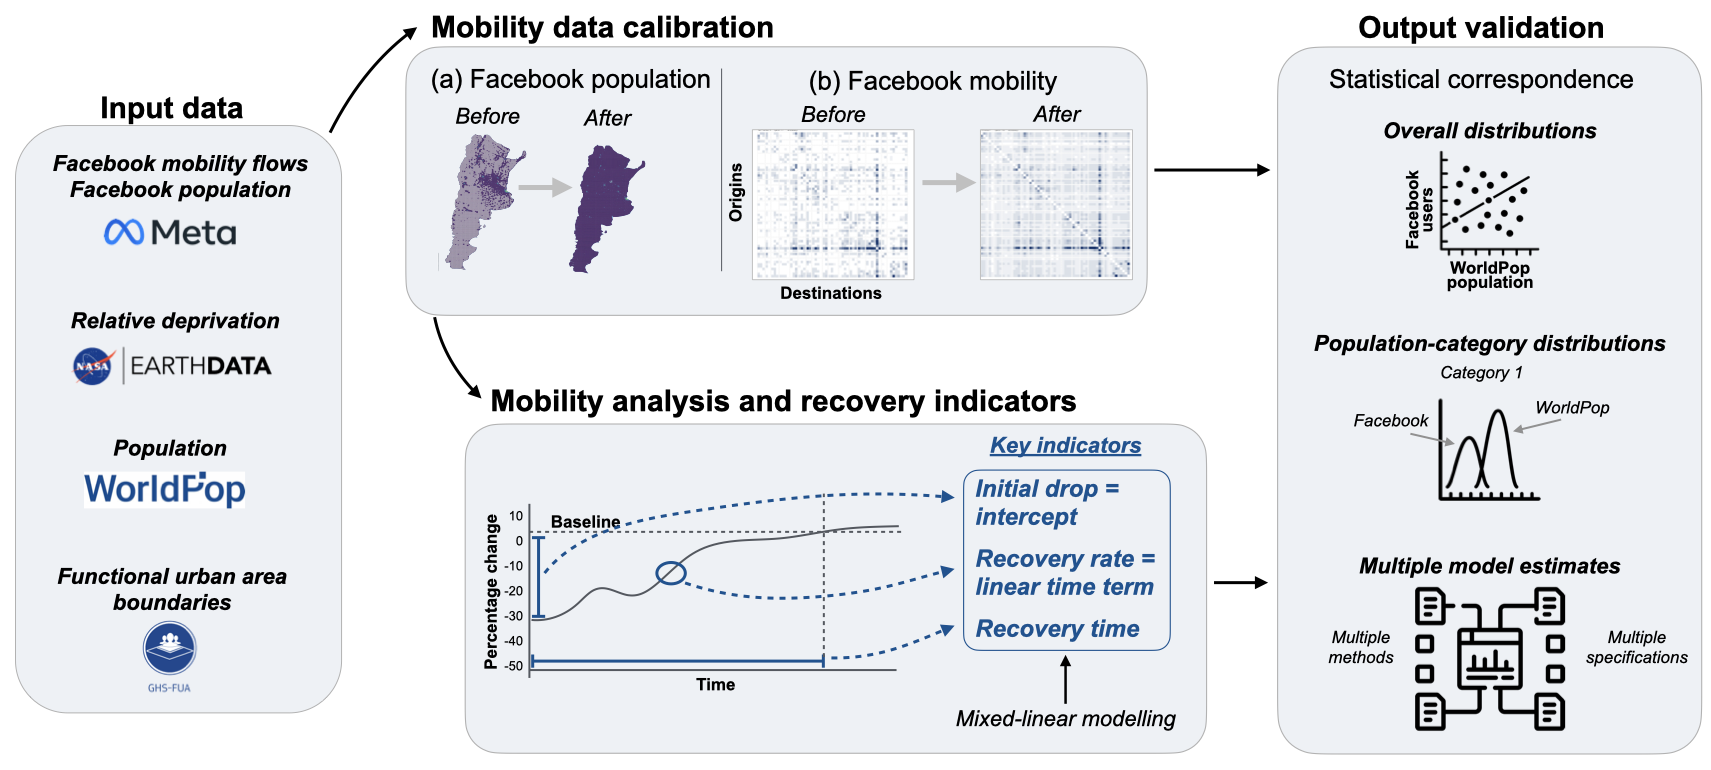
\includegraphics[width=0.9\linewidth]{figures/Fig-summary-diagram-r1.png}
\caption{Overview of our methodology. Detailed descriptions are provided in the Methods section. Facebook mobility and population data (Meta), relative deprivation (NASA), population estimates (WorldPop) and functional urban area boundaries (Global Human Settlement Layer) are used as inputs. Mobility data are calibrated to reduce spatial and temporal biases and analysed within each country using statistical models to estimate urban mobility recovery. Validation assesses consistency with WorldPop populations and robustness across calibration and model specifications.}
\label{fig-summary}
\end{figure}

We addressed important sources of common biases in mobile phone app data for our analysis. As most digital trace data, mobile phone data do not necessarily provide a representative picture of the overall population, largely because of algorithmic decisions and changes in users' engagement over time \cite{rowe2023big, barreras2024exciting, cabrera2025bias}. We know that Facebook suppresses population counts below 10 to protect users' privacy and that user engagement declined over time in our dataset. These adjustments may influence the observed patterns of mobility, especially in sparsely populated areas. To mitigate these issues, we applied a series of data corrections (see Figure \ref{fig-summary}). First, we modelled the Facebook user population data as a function of Worldpop population data to generate a complete spatial population surface. Second, we modelled the Facebook mobility data to estimate origin-destination flows that were suppressed by the Facebook algorithm. Third, we used the temporal median of the sum of active user counts divided by the sum of active user counts across all spatial units on a given day to normalise for fluctuations in Facebook user engagement over time. Full details of these procedures are provided in the Methods section, and Supplementary Table ST1 summarises the extent of data imputation. Supplementary Note SN1 reports external consistency checks of our findings, using official mobility and labour statistics from Buenos Aires, Colombia, Chile and Latin America.

\subsection*{COVID-19 led to lasting disparities in mobility patterns}

We first compared the change relative to baseline levels of mobility during the early pandemic in 2020, and once most restrictions were lifted in 2022, as shown in Figure \ref{fig-impact}. Boxplots display the percentage change distribution of areas based on population density and relative deprivation level categories, with a $y = 0$ line representing baseline levels. Scores above this line indicate increased mobility from pre-pandemic levels, while values below represent a reduction. 

\begin{figure}[h!]
\centering
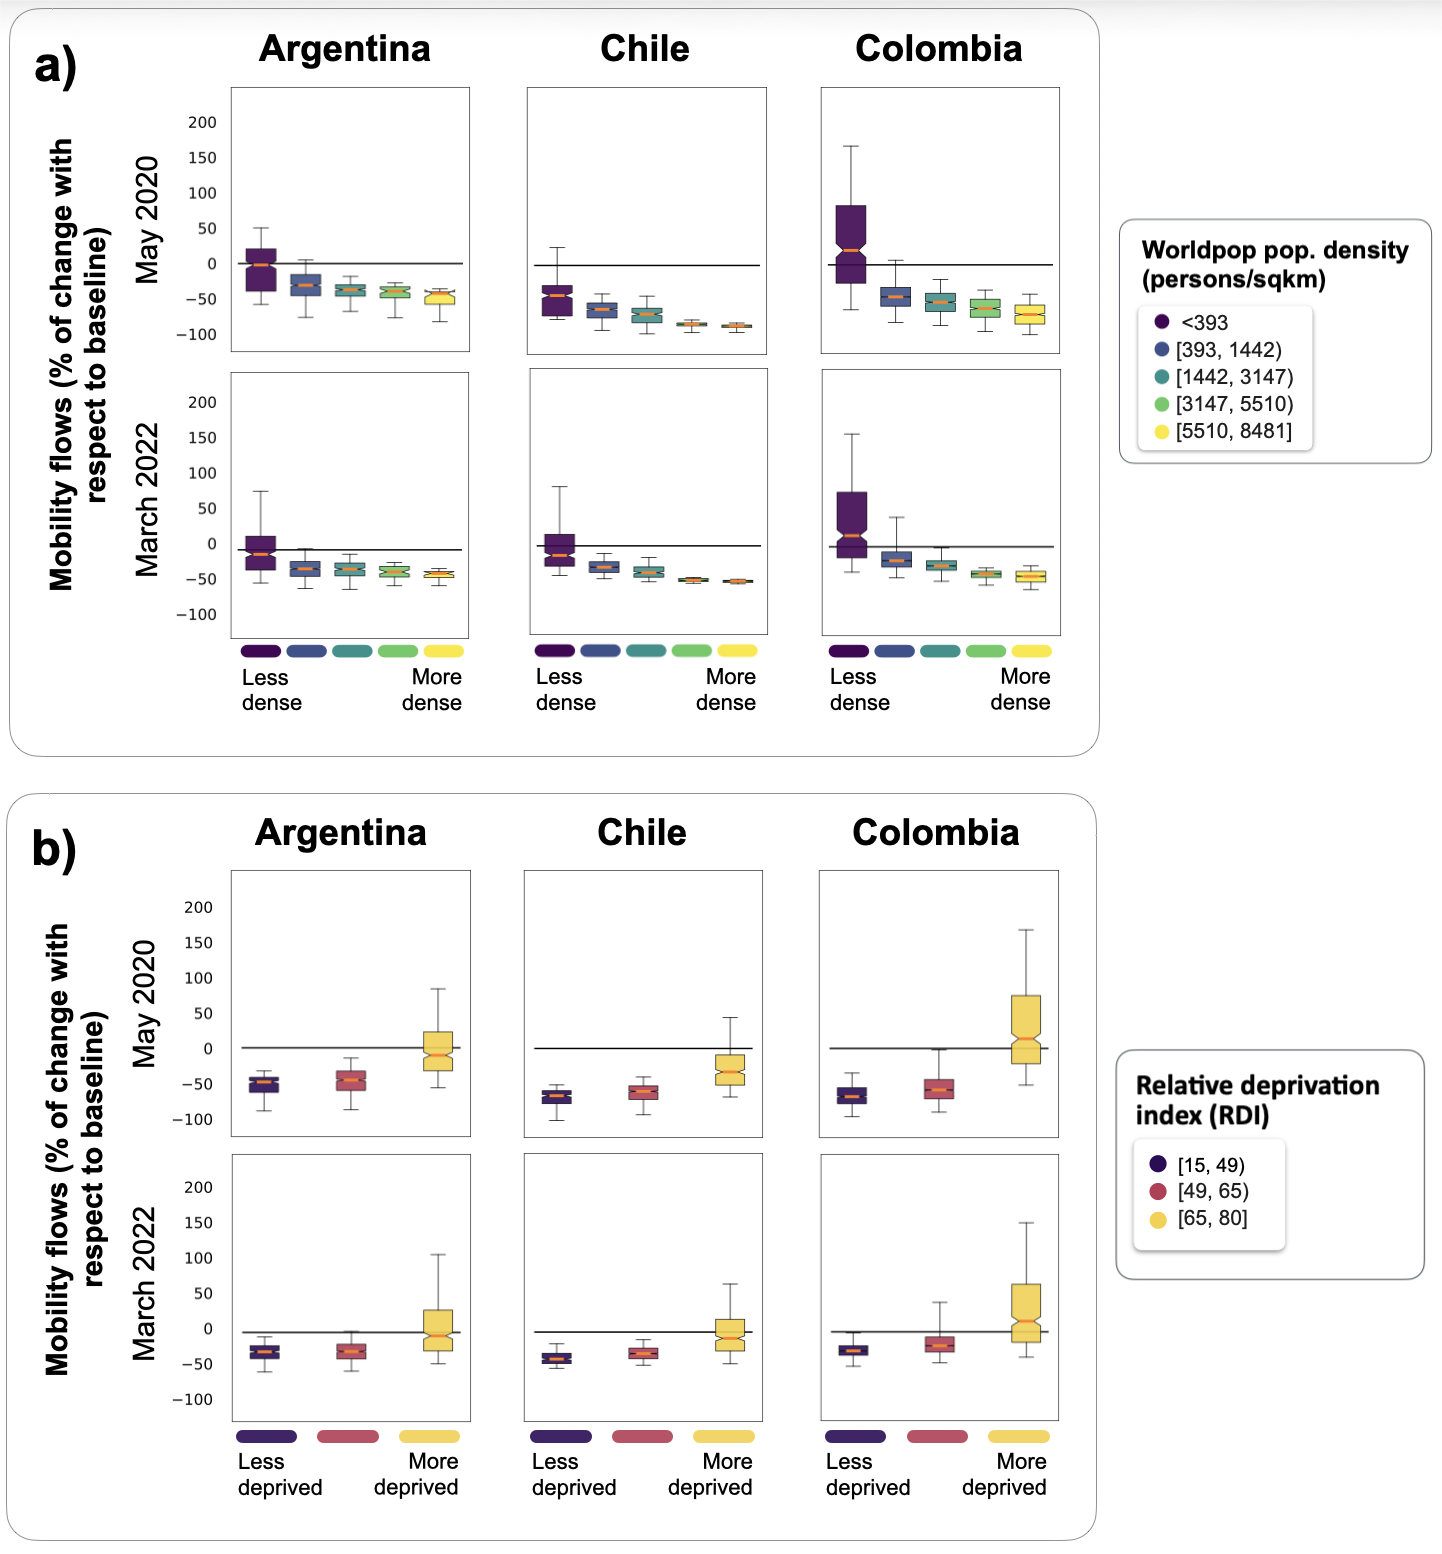
\includegraphics[width=0.9\linewidth]{figures/Fig-impact-design-r2.png}
\caption{Percentage change in mobility counts in May 2020 and March 2022, relative to the pre-pandemic baseline levels in Argentina, Chile and Colombia. Mobility flows are aggregated by area type, with areas classified along two independent dimensions used in the research design: population density and socioeconomic deprivation. Population density is used as a proxy for position along the rural–urban gradient within each country, following an established approach in the migration and settlement literature and in applied classification frameworks \cite{championhugo2004, rees1999internal, rees2017impact, GHSL19, UNpopulation25}. Socioeconomic deprivation is classified into three categories based on the Relative Deprivation Index (RDI) \cite{RDI2022}. The figure presents descriptive comparisons across these groups and does not include interaction effects between density and deprivation. Full details on the data, classifications and assumptions are provided in the Methods section.}
\label{fig-impact}
\end{figure}

The results consistently show larger and more persistent declines in mobility in high-density areas compared to low-density areas. This persistence of reduced mobility levels in high-density areas is a novel finding, suggesting that the COVID-19 pandemic led to significant behavioural mobility changes in cities which have endured over time. The consistency of such a pattern is remarkable taking place in all three Latin American countries in our sample, showing little discrepancy within countries (as shown by relatively narrow box plots). In contrast, low-density areas show mobility patterns closer to pre-pandemic levels and greater variability. The large variability is due to the small population bases in these areas, where minor fluctuations in movement can result in disproportionately large percentage changes. The patterns observed in Figure \ref{fig-impact} are also observed when the analysis is repeated using non-imputed mobility data (SF7), indicating that the conclusions are not driven by the data imputation process.

Our findings also evidenced enduring socio-economic disparities on the impact of the pandemic on mobility patterns. Prior research demonstrated that, early in the pandemic in 2020, a social gradient emerged, leading to sharper declines in mobility in less deprived areas compared to more deprived communities. We find that this social gradient effect has endured over time, as workers from more deprived areas are likely travelling as much (or more) as they used to prior to the outbreak of the COVID-19 pandemic - indicated by box plots stretching above baseline levels. These patterns are remarkably consistent across all three countries. This is despite differences in the initial extent of mobility decline across countries in 2020. Relative to baseline levels, initial reductions in mobility were larger in Chile (45-50\%) than in Colombia (40-45\%) and Argentina (25-30\%).


\subsection*{Early mobility declines during the pandemic shape long-term levels of mobility}

Discrepancies in the resilience of areas may underpin the observed differences in mobility levels. To quantify the resilience of areas, we model the trends of mobility recovery to pre-pandemic levels as a function of time. To this end, we decomposed the time series of the percentage change in mobility into trend, seasonal and residual components using a moving-average–based method. Robustness checks using alternative trend extraction techniques are reported in Supplementary Table (ST) ST2. The time series are displayed in SF10. We modelled the trend component as a function of time, stringency levels and attributes of the places of origin, including population density, relative deprivation and old-age dependency ratio (the latter category reported only in the Supplementary Information), in a mixed-effects modelling framework – see Methods section and ST3 for details.  Stringency levels are measured via the COVID-19 Stringency Index created by \cite{hale2021global}, which we include to assess the influence of changes in government restrictions on mobility. The index aggregates daily data on nine policy indicators including school and workplace closures, cancellation of public events, restrictions on gatherings and movement, public transport closures, stay-at-home requirements, international travel controls and public information campaigns. Specifically, the inclusion of the variables internal travel and mobility restrictions and stay-at-home into the stringency index allows us to control for restrictions on population movements during the COVID-19 pandemic.

Fourteen model specifications were fitted separately for each country. The full set of regression estimates is provided in ST4-9. Time and stringency index were strongly colinear (Pearson $r = -0.91$, $p < 0.01$); accordingly, Figure \ref{fig-re-combined} (a) and (b) reports estimates from time-only models, which were also favoured by the Akaike Information Criterion (AIC). Among all models, Model 6 generally yields the lowest AIC score, indicating the best overall fit. To assess robustness, we additionally estimated a Generalised Additive Model (GAM) specification (Model 8). Although the GAMs consistently produced lower AIC values, they show evidence of overfitting (high effective degrees of freedom for class-specific splines). GAM model outcomes are also reported in ST4-9.

\begin{figure}[!htbp]
\centering
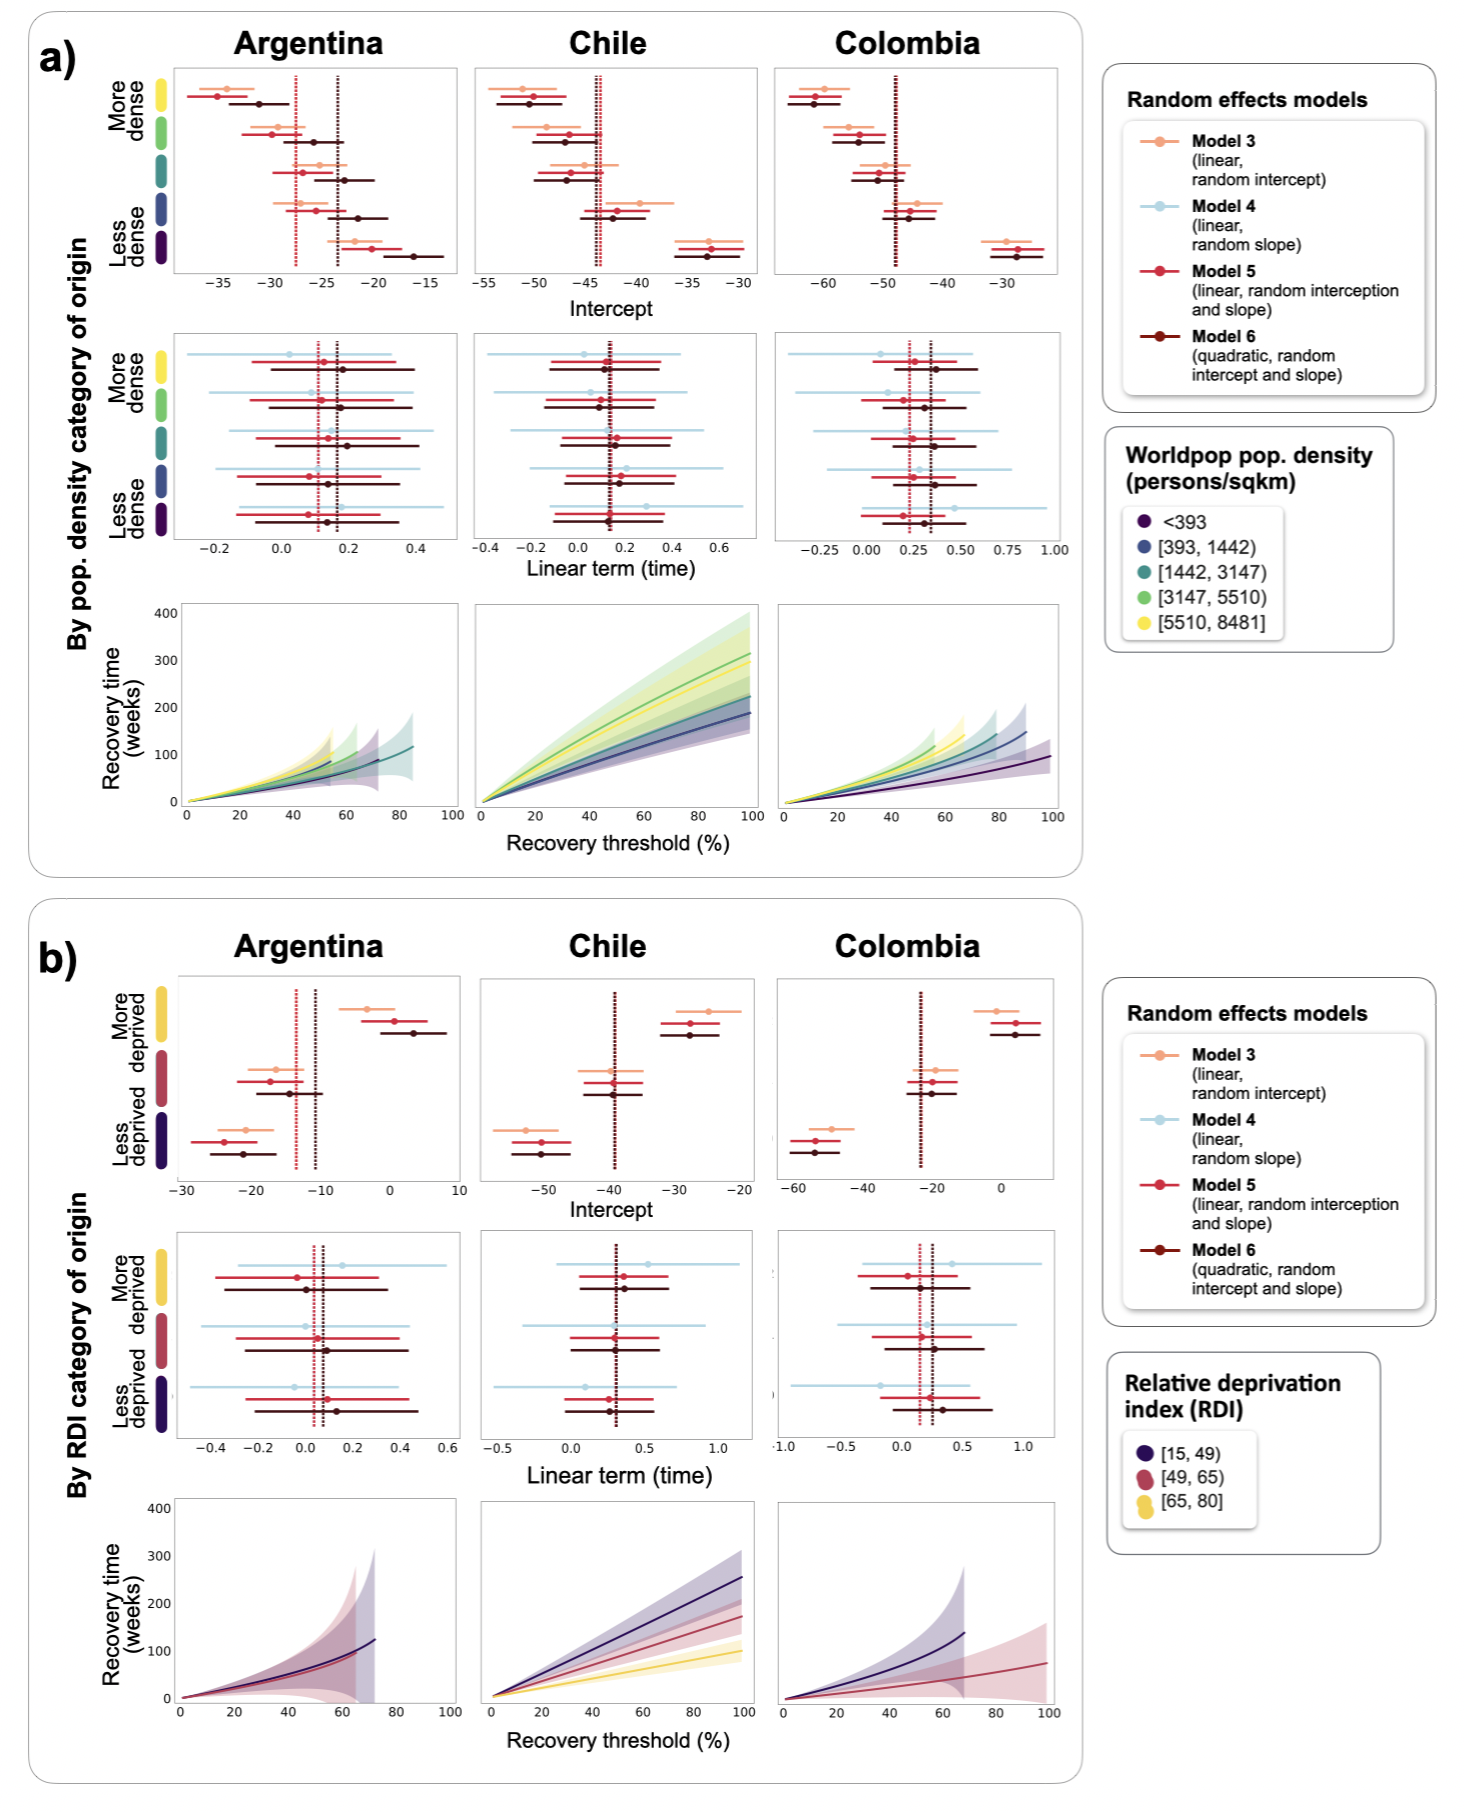
\includegraphics[width=0.9\linewidth]{figures/Fig-re-combined-design-quad-recovery-time-std-r2.png}
\caption{First and second row of each panel represent mixed-effects modelling estimates (random intercept and random linear time term); bars denote 95\% confidence intervals; colours encode different model specifications; vertical dashed lines represent the estimated values for fixed effects of the corresponding terms (i.e. intercept, linear time). The third row represents estimated recovery times at different thresholds. Panel (a) displays results by population density category and (b) by relative deprivation category.}
\label{fig-re-combined}
\end{figure}

The model estimates reported in Figure \ref{fig-re-combined} correspond to coefficients for intercept and time terms from Models 3-6 for population density (a) and deprivation (b). The intercept represents the estimated percentage decline in mobility during the week when Meta began producing mobility records, correcting for seasonality and noise. Negative scores indicate reductions in mobility levels, relative to the baseline period. The time term captures the linear component of the weekly rate of mobility recovery, relative to baseline levels. A time quadratic term was also included to capture variations in the pace of mobility recovery over time as reported in ST4-9 for Models 6 and 7. Model 7 includes random effects for the quadratic term. This adds complexity to our model, but it does not improve the estimation (higher AIC) and is often insignificant (p-value$>0.05$). Estimates from various model specifications evidence the consistency of our findings. Additionally, we also estimated mobility recovery times, reported in both panels (a) and (b); that is, the time taken (in weeks) for mobility to reach various thresholds based on pre-pandemic mobility levels. For low-deprivation groups in Argentina and Colombia, recovery times are not reported, as average mobility levels for these groups did not fall below the baseline during the observation period. The Methods and Supplementary Information (SI, section 4) describe how the recovery time estimates and uncertainty bands were computed. ST22-23 report recovery time estimates by country at four different thresholds (25\%, 50\%, 75\% and 100\%), and by population density or RDI category, computed according to mixed-effects Model 6 and to GAM-based Model 8. 

We highlight three main findings. First, the random intercept estimates are consistent with the evidence in Figure \ref{fig-impact} revealing a descending gradient across rural-urban and socioeconomic structures during early stages of the pandemic. Mobility declined the sharpest in highest-density and least-deprived areas, while low-density population and more deprived areas registered small declines. These estimates suggest that populations in affluent and more dense urban areas have more flexibility to adapt to early COVID-19 restrictions by reducing their mobility levels and turning to remote work. Poorer and less populated communities had less flexibility to transition to remote work. Although intercepts also differ across old-age dependency ratio categories, these differences do not form a systematic gradient across countries, so we only report them as part of the Supplementary Information (SF11; ST4–ST9).

Second, our regression estimates show differences in random intercepts but overlapping confidence intervals for the random time slopes. These results suggest that differences in mobility recovery across rural-urban and socio-economic gradients over time reflect differences in the magnitude of the initial mobility shock (intercepts), rather than in recovery rates (time slopes) following the initial COVID-19 outbreak. The identified patterns are consistently observed when using non-imputed data as input for the models, as shown in SF13, indicating that the findings are not driven by the imputation process. Recovery time estimates indicate a consistent grading across rural-urban and socio-economic structures. Higher density and less deprived areas display longer recovery times, indicating that mobility is estimated to take longer to reach pre-pandemic mobility levels. Differences in recovery times along rural-urban and socio-economic gradients are therefore driven by the magnitude of the initial mobility shock (captured by our intercept estimates), rather than by differences in recovery rates (captured by our time estimates). These effects are similarly observed across old-age dependency ratio categories, as reported in SF11 and ST4-9.

Third, recovery time estimates (Figure \ref{fig-re-combined} bottom panel) indicate longer recovery periods in mobility for higher population density and less deprived areas. The lowest population density areas in Chile are estimated to take 132 weeks to achieve 100\% of observed pre-pandemic mobility levels, but as much as 201.87 weeks in the highest density areas. The differences in recovery times are consistent across countries. Yet, wide variability exists between them. Chile systematically displays the longest estimated recovery times. They tend to be twice as large as those recorded for Argentina and Colombia, where stringency measures implemented at the outset of COVID-19 triggered a rise in mobility in the low density areas and highly deprived communities, exceeding pre-pandemic levels (SF10).

Overall, our findings indicate a strong persistence of the immediate COVID-19 mobility shock. They suggest that post-pandemic mobility disparities reflect the immediate shock of COVID-19, rather than differences in recovery rates across communities. COVID-19 appears to have led to new mobility regimes reflecting pre-existing urban and socio-economic inequalities. Our findings indicate that the unequal mobility declines observed in March 2020 across rural-urban and deprivation gradients persisted well beyond the lifting of restrictions and vaccine rollout, lasting at least two years after the onset of COVID-19.


\subsection*{Dense urban cores report persistent reductions in net mobility outcomes}

Next, we examine the resilience of high-density urban core areas as attractors of daily mobility. Prior work identified a hollowing out of cities since the COVID-19 outbreak, or ``doughnut effect'', with a net loss of daily mobility into urban centres \cite{ramani2024working}. However, such evidence is limited outside the US context \cite{ramani2024working, gonzalez2023donut}. We analysed the evolution of netflows (i.e. inflows minus outflows) in relation to pre-pandemic levels. We measured netflows for all urban cores in the country, and only for the capital's urban core (i.e. Buenos Aires, Santiago and Bogotá), to assess the extent to which flows to the capital may influence the results. We used Functional Urban Areas (FUAs) boundaries from the GHSL to define urban regions \cite{ceu.jrc.2019}, and for each urban region, we distinguish the urban core as the most densely populated spatial unit of analysis (the densest Bing tile within the FUA, see Methods), which effectively contains the CBD. 

Figure \ref{fig-fuasflows} displays the evolution of these netflows by population density category. We seek to assess the extent of population loss in urban cores due to mobility and its durability since the onset of COVID-19. We evaluate if urban cores in Latin American countries recorded declines due to mobility redistributing people to moderate population density areas (suburbanisation); to low-density areas (counter-urbanisation); or both. In Argentina, only the area corresponding to the urban core in Buenos Aires is classified in the highest density category, so no mobility interactions with other high-density areas are captured when analysing just the capital's urban core; hence, no yellow curve for the first panel in Figure \ref{fig-fuasflows} is reported. We used a mixed-effects modelling framework to analyse the time series in Figure \ref{fig-fuasflows} and for robustness, we also used a GAM model (results reported in ST10-21). The model results are consistent when using imputed and non-imputed mobility data, as demonstrated in SF14. We then estimated recovery times at multiple thresholds. These recovery times show remarkable consistency when estimated according to Model 6 and Model 8 (see ST24-25). According to our models, netflows to urban cores did not recover in some areas and as a result, recovery times could not be estimated for those areas.

%When the baseline netflow is positive, a negative percentage change between -100\% and 0\% indicates that the netflow decreases compared to the baseline but remains positive. Conversely, when the baseline netflow is negative, a percentage change between -100\% and 0\% suggests that the netflow remained negative during the crisis, though its absolute value was smaller than in the baseline period.

\begin{figure}[h!]
\centering
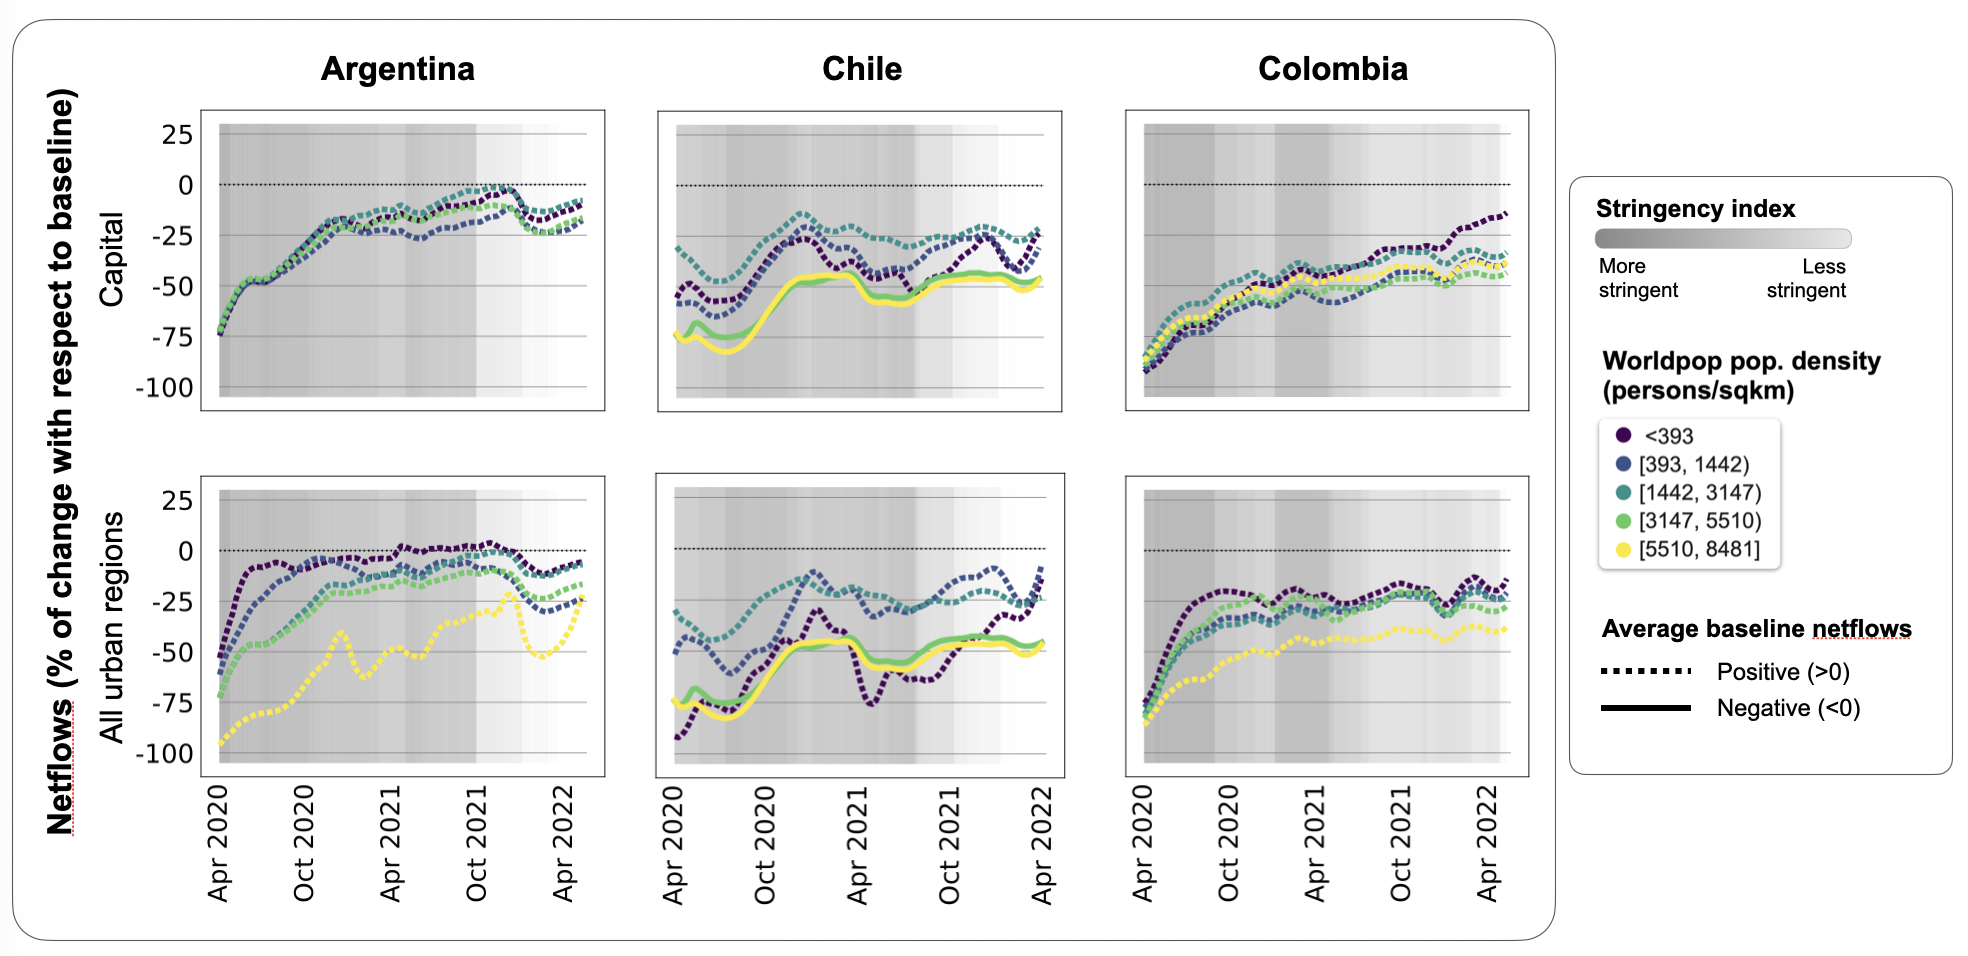
\includegraphics[width=\linewidth]{figures/Fig-fuas-netflows-simpler-no-baseline-r2.png}
\caption{Evolution of netflows for urban cores corresponding to the capital urban region and all urban regions (defined as Functional Urban Areas), by population density category for Argentina, Chile and Colombia, April 2020 to May 2022. Netflows are expressed relative to pre-pandemic baseline levels. Dashed and solid lines indicate, respectively, positive or negative pre-pandemic netflows on average.}
\label{fig-fuasflows}
\end{figure}

Our findings suggest a prevalent pattern of reduced netflows for urban cores following the enforcement of COVID-19 restrictions. Dashed lines indicate that netflows in urban cores incoming from other areas were positive pre-pandemic. However, the negative relative change since the COVID-19 outbreak reveals a reduction in the magnitude of these netflows. This reduction has predominantly become less acute over time across the rural-urban hierarchy in all three countries, but it remained below pre-pandemic levels following the lifting of COVID-19 restrictions in May 2022. These patterns reflect that while mobility inflows into core areas continued to exceed outflows, they shrank resulting in a smaller net balance. In Argentina and Chile, particularly in the capital city of Buenos Aires and Santiago, patterns of negative netflows are consistent with systematic evidence of net population losses due to internal migration in these metropolitan centres over the last two decades \cite{rowe2013spatial, vignoli2019efectos, rodriguez2022migracion}.


\section*{Discussion}

We assessed the durability of changes in mobility patterns across rural–urban and socio-economic gradients in Latin American countries from the beginning of the pandemic outbreak in March 2020 and following the rollout of vaccines and relaxation of lockdown measures in May 2022. Prior work showed that the pandemic resulted in large reductions in mobility levels in high-density urban areas and least deprived communities, reflecting reductions in commercial activity in urban areas, and a higher representation of affluent communities in jobs with higher potential for remote working \cite{bartik2020jobs, Zhou26}. Yet, existing evidence has focused on the immediate impacts of COVID-19 during early 2020 and on the restructuring of mobility patterns in more developed countries. We contribute to expanding this work by investigating the evolving impacts of COVID-19 on mobility beyond their initial aftermath extending to the second year of the pandemic in less developed countries.

We find evidence of sustained reductions in mobility levels in high-density urban areas and among the least deprived communities. These declines, first observed in the early months of the COVID-19 pandemic, persisted two years later, despite widespread vaccine rollout and the lifting of lockdown measures. We also find a sustained reduction of net balance of mobility flows in core urban areas. Historically, cities are critical engines of innovation, economic growth and prosperity \cite{Glaeser10}, enabling the emergence of agglomeration economies and facilitating knowledge exchange \cite{storper2004}. Our findings suggest that some of these benefits may have diminished. COVID-19 accelerated the adoption of technologies, online services and remote working at an unprecedented scale, reducing the need for physical co-location and eroding the vibrancy of urban centres \cite{Alexander21}. As people engage in virtual activities, planning strategies should be reoriented to repurpose existing infrastructure and develop new required infrastructure, accommodating the ways in which people move and use cities in a post-pandemic world. Transport systems, for example, may need to be redesigned to accommodate less frequent trips to core urban areas, and less frequent but longer-distance commuting trips from lower-density areas to employment centres. Digital infrastructure in more remote areas may require an upgrade to accommodate improved connectivity and seamless virtual data transfers.

Our findings reveal persistent differences in mobility recovery trends across rural-urban and socio-economic gradients. We find that disparities in the initial impact of the COVID-19 pandemic on mobility across population groups largely account for the sustained differences in recovery trajectories. While the magnitude of the initial shock varied significantly across rural-urban and socio-economic groups, the subsequent rates of mobility recovery have remained relatively uniform over the long term. Higher-density and less deprived areas displayed shorter overall recovery times compared to lower-density and more deprived areas. Disparities in mobility are likely driven by differences in the nature of employment \cite{ILO21} across rural-urban and socio-economic groups. This interpretation is supported by external evidence based on official mobility statistics and labour and household surveys from Latin America and the Caribbean \cite{OMSV2026BA, DANE2025, ILO2023PanoramaLaboral, BertranouGontero2024LACWork}. These sources are consistent with our finding that daily mobility volumes have not fully returned to their pre-pandemic baseline and indicate that remote work has remained above pre-pandemic levels. However, these patterns may be about to change following recent shifts in employers' attitudes towards remote working, such as the presidential actions of the US government, with mandates for more days in the office \cite{WhiteHouse2025Return, CIPD2025LMO}. Overall, our findings suggest that government efforts to reduce mobility disparities across rural-urban and deprivation divides should prioritise mitigating the initial shock of pandemics, as recovery trajectories tend to progress at similar rates across groups once the immediate disruption has passed.

Despite our robustness and validation tests, key challenges should be considered when interpreting our results, which are better understood as plausible hypotheses that can guide future research rather than as definitive causal claim. First, limitations related to the use of aggregated mobile-phone–derived mobility indicators. These data are generated from a non-random sample of users providing variable coverage across space and time, and potentially under-representing population groups with lower smartphone access, limited digital connectivity or higher privacy opt-out rates \cite{cabrera2025bias}. As such, inferred mobility changes may not fully reflect the behaviour of all sociodemographic groups, particularly in more disadvantaged areas. Second, the pre-pandemic baseline used to define reference mobility levels is limited to a 45-day period provided by Meta and therefore does not capture longer-term seasonal variability. While this baseline precedes mobility restrictions and accounts for day-of-week effects, it may affect estimates of the absolute magnitude of the initial mobility drop, though relative recovery trajectories are less sensitive to this limitation. Third, our data do not provide information on modal split, limiting inference on the persistence of changes in specific transport modes, such as walking, cycling or micromobility \cite{zhang2023impacts, KaganCapkin25}. Fourth, observed mobility changes reflect outcomes rather than travel motivations, constraining our ability to distinguish behavioural adaptation from mobility reductions driven by affordability, service availability or labour informality. Fifth, our analyses are observational and conducted at an aggregate spatial scale, so associations between mobility recovery and city characteristics should not be interpreted as causal and may be influenced by unobserved factors, such as changes in transport supply or concurrent economic shocks. Finally, while external benchmark data for population counts are available consistently across countries, comparable external movement data are not generally available at the spatial and temporal scale required to validate mobility patterns across rural-urban and socioeconomic gradients. These limitations motivate future work combining digital trace mobility data with external validation sources and complementary data to assess representativeness, modal split and causal mechanisms.

The evidence reported here potentially has important social equity implications by exacerbating pre-existing disparities in Latin America. The region is among the most unequal regions in the world \cite{WIReport22}. The bottom 50\% of the Latin American population holds only around 10\% of wealth\cite{WIReport22}, and is likely to face a disproportionately high social burden due to a more limited capacity to work remotely and a continued reliance on physical mobility for accessing employment and services. This entails financial and non-financial opportunity costs, such as transport fares and travel time. By contrast, the top 10\% of the population, which holds approximately 55\% of wealth\cite{WIReport22}, may continue to reduce travel due to greater flexibility in work arrangements and access to digital alternatives. As a result, uneven mobility recovery across socio-economic groups may function as a mechanism through which pandemic-era disruptions become embedded into long-standing patterns of inequality and spatial mismatches between residence and opportunity, with potential consequences for labour market participation, educational attainment and access to essential services. 

These sustained mobility changes also have important implications for Latin American cities and their governance. Sustained suppression of mobility into urban cores risks undermining commercial activity and overall urban vibrancy, particularly if higher-income populations continue to travel less frequently to central areas. These dynamics may reinforce already emerging patterns of urban centre decline in some large Latin American cities, as we saw in European cities during the 1970s and 1980s \cite{THORSTEN}. In Latin America, where metropolitan governance is often fragmented across municipalities and fiscal capacity for large-scale interventions remains limited \cite{un2022world, inostroza2013urban, fay2017rethinking, irazabal20governance}, the persistence of depressed urban core activity highlights the need for targeted, context-specific responses, rather than broad calls for inclusive or sustainable mobility. Policies prioritising affordable and reliable public transport connections to central employment and service hubs, particularly during peak hours and along high-demand corridors, may be more effective than uniform system-wide measures \cite{rivas2019urban, guzman2022effects}. More broadly, the observed heterogeneity in recovery trajectories underpins the importance of metropolitan-scale coordination in transport and urban planning, as city-level responses alone may be insufficient to address persistent shifts in urban activity patterns \cite{duque2021institutional}. In this scenario, near real-time mobility data offer a valuable tool for identifying emerging signals of urban decline and supporting adaptive, evidence-based policy interventions in contexts where traditional data sources remain delayed or incomplete.


% Key points to get across
%    - Although diminished, the early reduction in mobility in highly dense urban areas and the least deprived continued after two years the initial COVID-19 outbreak
%        - Implications: hibrid working and 
%    - The initial gap in reductions in mobility levels across the rural-urban and deprivation structures has persisted over time, reflecting limited differences in the rate of mobility recovery and longer recovery times in highly dense urban areas and less deprive communities.
%        - Looking at future recovery
%    - Net flows in core urban areas have systematically reduced and remained below pre-pandemic levels.
%        - Implications in terms of loss of attractiveness / hibrid working / more sustainable cities. 
%    - Methodological contribution on calibrating the data, correcting for biases



% Assuming a linear trend in mobility recovery, we find that highly dense urban areas take up to 2.5 times longer to recover than sparsely populated areas. In sparsely populated areas, mobility recovered faster as residents rely on travel to access essential services, reflecting that movement is a necessity rather than a choice. Similarly, deprived areas tend to recover faster than affluent areas, with the former sometimes experiencing little to no decline in mobility. More deprived populations are likely to work in occupations that require in-person presence, leaving them with fewer opportunities for remote work. Affluent populations, on the other hand, are more likely to hold office-based jobs that allow for remote work, reducing the immediate need to resume regular movement \cite{ILO21}.

% Our findings indicate that the resilience of different areas to the impact of the pandemic is mainly determined by the severity of the initial shock, rather than differences in their recovery rate. Since the recovery rate (slope of linear trend) is similar across population groups, all areas followed parallel recovery trajectories once mobility began rebounding. However, areas that experienced a more severe initial decline (intercept) had a longer road to recovery because they started from a lower point. This suggests that strengthening resilience to shocks such as pandemics requires strategies that minimise the severity of the initial impact, as recovery patterns tend to follow a similar trajectory across different areas. 

% Two years after the initial outbreak, daily movement into urban cores has not fully recovered in most cases, with a particularly sharp decline in Chile. The advantages of agglomeration economies, which include fostering innovation and growth by clustering talent and resources \cite{storper2004}, have historically driven urban resilience, particularly in the context of pandemics \cite{Glaeser10}. However, COVID-19 has accelerated the adoption of technologies that reduce the need for physical co-location at an unprecedented scale \cite{Alexander21}. As more people engage in virtual activities such as remote work, online shopping or digital collaboration, there is a need to rethink planning, infrastructure, and economic strategies to sustain urban vitality in a post-pandemic world.

\section*{Methods}

\subsection*{Data}

\subsubsection*{Facebook Movement During Crisis}

We used anonymised aggregate mobile phone location data from Meta-Facebook users to capture population movements for Argentina, Colombia and Chile, covering a 26-month period from April 2020 to May 2022. We used the Facebook Movement During Crisis datasets created by Meta and accessed through their Data for Good Initiative (\href{https://dataforgood.facebook.com}{https://dataforgood.facebook.com}). The data are built from Facebook app users who have the location services setting activated on their smartphone. Prior to releasing the datasets, Meta ensures privacy and anonymity by removing personal information and applying three privacy-preserving processes \cite{Maas19}. First, Meta adds a small, undisclosed amount of random noise to prevent the determination of precise counts for these areas.
Second, they apply spatial smoothing, using inverse distance-weighted averaging, to create a smoother data surface. Third, they drop small counts to exclude records data counts below 10.

The Facebook Movement datasets provide information on the aggregated number of Facebook app users moving between pairs of locations from April 2020 to May 2022 during the COVID-19 crisis period. The data is spatially aggregated into tiles according to the Bing Maps Tile System developed by Microsoft \cite{MicrosoftBingMaps}. The Facebook Movement data are spatially aggregated into Bing tiles at resolution level 10 for Argentina and Chile, and level 12 for Colombia, which correspond to squares of 19.57 $\times$ 19.57 km and 4.89 $\times$ 4.89 km, respectively. The data are temporally aggregated into three daily 8-hour time windows which are 00:00-08:00, 08:00-16:00 and 16:00-00:00, Pacific Time (PT). Since the Meta data are released only in these pre-aggregated 8-hour intervals, analysis at lower temporal resolution is not possible. The time windows translate to 05:00-13:00, 13:00-21:00, 21:00-05:00 for Argentina and Chile; and 03:00-11:00, 11:00-19:00, 19:00-03:00 for Colombia. For each time window, the origin location of a user is defined as the most frequently visited location in the previous time window, while the destination location is the most frequently visited location in the relevant time window.

In addition, each dataset includes baseline movement counts, which represent the estimated number of people moving before COVID-19. These baseline counts provided by Meta are calculated based on a 45-day period ending on March 10, 2020, using the average for the same time of day and day of the week within this period. For example, Meta calculates the baseline for the 00:00–08:00 (PT) window on Mondays by averaging all Monday records for that time window across the 45-day period. Further details about the baseline can be found in \cite{Maas19}.

Due to the small-count dropping privacy measure, movement counts during both the crisis and baseline periods are excluded if they fall below 10. However, even when counts are not reported, the datasets consistently provide the percentage change in movement counts relative to the baseline. This percentage change, denoted as $y^{\%}_{ijdt}$, is computed as follows \cite{Maas19}:

\begin{equation}
y^{\%}_{ijdt} = \dfrac{y^{c}_{ijdt} - y^b_{ijdt}}{y^b_{ijdt} - \varepsilon}\times 100.
\end{equation}

Here, $y^c_{ijdt}$ and $y^b_{ijdt}$ represent the crisis and baseline movement counts, respectively, between origin tile $i$ to destination tile $j$ on day $d$ and during time window $t$. For the baseline values $y^b_{ijwt}$, the subindex $w$ denotes the day of the week corresponding to day $d$, as the baseline values are recorded by weekday, not by specific date. A small constant $\varepsilon$, usually set to 1, is added to the denominator to avoid division by zero \cite{Maas19}.

\subsubsection*{Facebook Population During Crisis}

We also used the Facebook Population During Crisis datasets. Like the Facebook Movement data, these datasets cover a 26-month period from April 2020 to May 2022 and provide information on the number of active Facebook users at specific locations during the crisis period. The Facebook Population data for Argentina, Chile and Colombia are spatially aggregated into Bing tiles at resolution level 11 for Argentina and Chile, and level 12 for Colombia, which correspond to 9.78 $\times$ 9.78 km and 4.89 $\times$ 4.89 km tiles respectively. The Facebook Population data is released in pre-aggregated 8-hour time windows. A user's location is defined as the most frequently visited location within each 8-hour time window. Similar to the Facebook Movements datasets, the Population datasets include baseline counts, calculated by averaging values for the same day of the week and time of day over the 45-day pre-pandemic baseline period.

The same privacy-preserving techniques are applied to the Facebook Population datasets.
As a result, population counts during both the crisis and baseline periods are excluded if they fall below 10. However, the datasets consistently report the percentage change in active user counts relative to the baseline. For tile $i$, day $d$ and time window $t$, the relative change in active user counts $p^{\%}_{idt}$ is computed as:

\begin{equation}
   p^{\%}_{idt} = \dfrac{p^{c}_{idt} - p^b_{iwt}}{p^b_{iwt} - \varepsilon}\times 100, 
\end{equation}

where $p^c_{idt}$ and $p^b_{iwt}$ represent the crisis and baseline active user counts at tile $i$ on day $d$ and during time window $t$. Once again, the subindex $w$ in baseline values $p^b_{iwt}$ denotes the day of the week corresponding to day $d$, and $\varepsilon$ is a small constant usually set to 1, added to the denominator to avoid division by zero \cite{Maas19}. Through the paper, we use the term ``Facebook population'' in reference to the number of active Facebook app users.

\subsubsection*{Meta-Facebook data pre-processing}

We only included Facebook data for one time window per day: 08:00–16:00 Pacific Time (PT) corresponding to 13:00–21:00 in Argentina and Chile, and 11:00–19:00 in Colombia. This time window is used to capture daily mobility. Including data for the three time windows in the datasets could result in movement in opposite directions cancelling out when aggregating by day, and preventing us from capturing any meaningful patterns. To reflect our focus on one time window, we can drop the subindex $t$.

As a pre-processing step, we ensure that both the Facebook movement and population data are aligned in terms of spatial resolution for each country. All analyses at the country level are produced at a consistent spatial resolution. Since the Facebook Population datasets are generally released at a finer spatial resolution, we re-aggregate them to match the spatial resolution of the Facebook Movement data. We retain the Bing-tile geography as our unit of analysis because it provides the finest, most spatially standardised and cross-country comparable unit available in the Meta data. Aggregating or disaggregating to alternative areal units would require an additional estimation step, which could introduce further uncertainty and not remove the general modifiable areal unit problem \cite{openshaw83}.

\subsubsection*{Worldpop population data}

We used data from Worldpop \cite{tatem2017} to classify our spatial units by population density category and to estimate missing baseline values in the Facebook population data.
We used gridded population data at a resolution of 1km$^2$ in raster format. We performed a spatial join of the Facebook spatial units (Bing tiles) with the gridded population data and computed the sum of Worldpop populations corresponding to each of the Facebook spatial units. In addition, we used the age-disaggregated WorldPop layers to compute the old-age dependency ratio in each spatial unit (defined as the percentage of the population aged 65 and over), which we used to examine differences in mobility patterns by age structure. The results of this analysis by age structure are reported in the Supplementary Information.

\subsubsection*{Socioeconomic deprivation data} 

We used the Global Gridded Relative Deprivation Index (GRDI), Version 1 (GRDIv1) \cite{RDI2022} dataset as a measure of relative socioeconomic deprivation. The index captures multiple structural dimensions, which are further detailed in Supplementary Table ST2. The GRDI data is available via NASA's Socioeconomic Data and Applications Centre (SEDAC) at a spatial resolution of 30 arc-seconds, or 1 km$^2$ approximately. The index takes values between 0 and 100, where 0 represents the lowest level of deprivation and 100 the highest. We performed a spatial join of the Facebook spatial units and the gridded relative deprivation data. We computed the average RDI corresponding to each of the Facebook spatial units.


\subsection*{Addressing missing data through data imputation} 

A challenge in analysing the Facebook population counts and movements is the absence of records for small counts. These records are removed to ensure privacy and anonymity. Yet, they may impact the analysis as the Facebook datasets include a high number of missing records, as shown in ST1. Missing values display a strong spatial pattern (see SF1). As such, sparsely populated spatial units or small active Facebook user populations could potentially be under-represented in the analyses. Simply removing the missing records from the analysis could lead to geographically biased results \cite{afghari2019}. To address this, we designed a data processing method for missing data imputation. After imputation, the alignment between Facebook-derived population distributions and WorldPop benchmarks improves, particularly across population density and deprivation categories (see SF9), indicating that the corrected data offer a more representative input for subsequent mobility analyses. Importantly, the substantive findings of the study remain consistent when obtained from imputed data and from data without imputation, demonstrating that our conclusions are not an artefact of the imputation procedure (see SF7, SF13 and SF14 for further details).

\begin{figure}[h!]
\centering
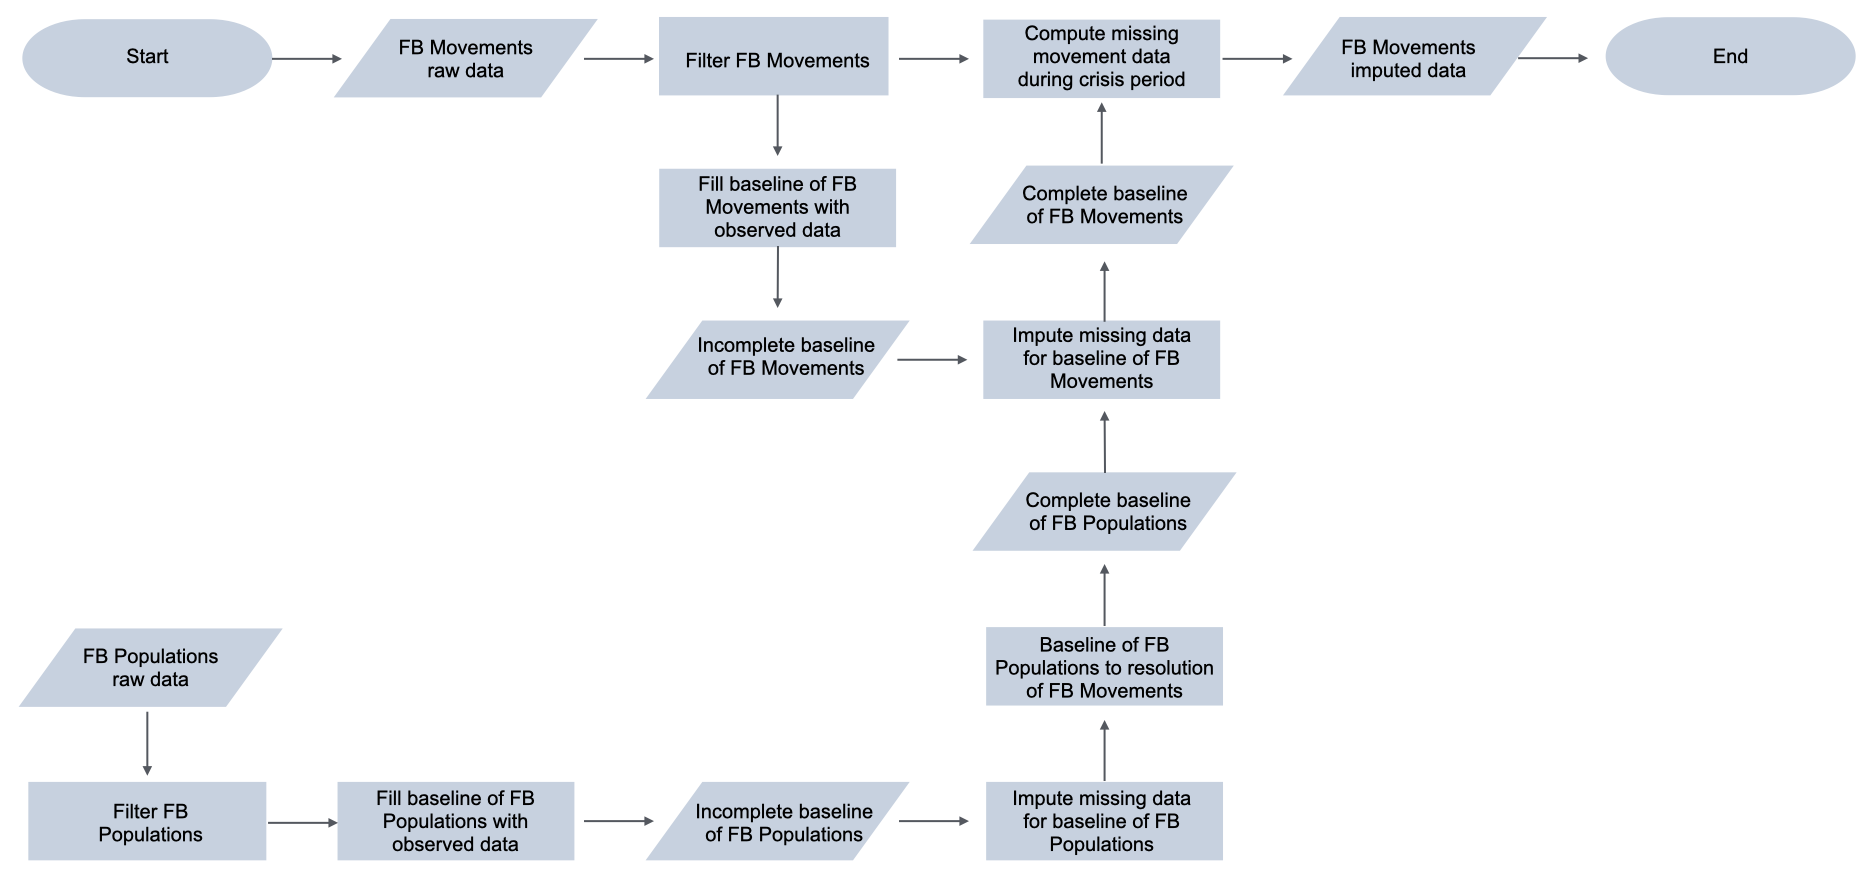
\includegraphics[width=\linewidth]{figures/workflow-diagram-r1.png}
\caption{Workflow diagram for the data imputation method. Rectangular boxes represent processes or actions, rhomboid shapes indicate inputs or outputs, and oval shapes mark the start and end of the workflow.}
\label{fig-dataimputation}
\end{figure}

\subsubsection*{Imputing Facebook Population data}

First, we identified all the baseline values reported in the Facebook Population datasets, which form the basis for creating a new dataset that includes all available baseline information. Following \cite{duan2024}, we used linear models to estimate the missing Facebook population baseline counts based on Worldpop population data. These models are fitted using ordinary least squares regression, with Worldpop data as the explanatory variable and the available baseline counts from the Facebook Population dataset as the dependent variable. The estimation process and its accuracy are illustrated in SF2-4 for Argentina, Chile and Colombia, respectively. 

We then used the complete baseline of Facebook population counts to compute missing Facebook population counts during the crisis period. This is possible because, as mentioned above, Meta reports the percentage change in the number of counts with respect to the baseline $p^{\%}_{id}$, even if the counts are not reported due to numbers below 10. The number of missing records and the extent of Facebook population data imputation are reported in ST1.

\subsubsection*{Imputing Facebook Movement data}

The imputation of Facebook Movement baseline values is done through the use of spatial interaction modelling \cite{rowe2024spatial}. The number of missing records and the extent of data imputation are reported in ST1. We used baseline movement counts $y^b_{ijw}$ between pairs of origin $i$ and a destination $j$ tiles on weekday $w$, and modelled these counts as a function of the Facebook population count at the origin tile on the same weekday, the Facebook population count at the destination on the same weekday and the distance between origin and destination.
We also included indicator variables to capture the day of the week.
Mathematically, this model can be expressed as: 

\begin{equation}\label{eq:sim}
\mu^b_{ijw} = \beta_0 + \beta_1p^b_{iw} +\beta_2p^b_{jw} + \beta_3d_{ij} + \beta_4w + \varepsilon
\end{equation}

where: $\mu^b_{ijw} = E[y^b_{ijw}]$ is the expectation of the flow of people from tile $i$ to tile $j$ on the weekday $w$ during the baseline period; $\beta_0$ is an intercept, $p^b_{iw}$ and $p^b_{jw}$ are the Facebook population counts at the origin and destination on weekday $w$ during the baseline period, $d_{ij}$ is the distance between origin and destination, $w$ is a series of indicator variables capturing the day of the week, and $\beta_{0,1,2,3,4}$ are model parameters to be estimated from the observed data. The error term is denoted by $\varepsilon$.

To estimate the model parameters, we used a censored log-normal model specification, with the logarithm of the origin population, destination population and distance as predictors. This specification reflects the fact that missing Facebook movement counts arise because values below 10 are censored for privacy reasons. SF 5 demonstrates the high correlation between the counts for observed flows and those predicted according to the spatial interaction model as specified in equation \eqref{eq:sim}. SF6 provides additional validation of the spatial interaction model used to estimate missing baseline Facebook movement counts. This figure illustrates the Facebook population at the origin and destination of each flow during the baseline period, considering the imputed Facebook population baseline data. The results demonstrate that, for both observed and predicted data, high-volume flows typically occur between highly populated origin and destination locations, aligning with expected patterns.

We computed missing Facebook movement counts during the crisis period by considering the imputed baseline of Facebook movement counts and the percentage change in the number of counts with respect to the baseline, which is reported in the Facebook Movement datasets even when the count is not reported due to its low value. The number of missing records and the extent of Facebook Movement data imputation are reported in ST1.

\subsection*{Addressing temporal fluctuations in data coverage}

A second data challenge arises from temporal fluctuations in the number of active Facebook users. To address this, we applied correction factors and time series smoothing to eliminate the fluctuations in the daily number of observations, ensuring that the representativeness of Facebook data across spatial units remains stable during the study period. The steps of our data-processing workflow are described next.

\subsubsection*{Applying correction factors}

The total number of active users within a given time window shows daily fluctuations due to limitations in Internet connectivity and user data access options \cite{Maas19}. Following \cite{yabe2020} and \cite{duan2024}, we applied a correction factor to mitigate the potential impact of these daily fluctuations on the results, since they could mask the mobility trends. This approach assumes that the representativeness of Facebook data across spatial units remains consistent throughout the study period.

The adjusted number of movements between tile $i$ and tile $j$ on day $d$, $y'_{ijd}$ was obtained as:

\begin{equation}
y'_{ijd} = k_d \times y^c_{ijd}
\end{equation}

where: $y^c_{ijd}$ is the original number of movements between tiles $i$ and $j$ on day $d$ during the crisis period and $k_d$ is a correction factor computed as the median of the sum of active user counts across all days $d$ divided by the sum of active user counts across all spatial units on day $d$. Mathematically,

\begin{equation}
k_d = \dfrac{\mbox{med}_d\big(\sum_i{p^c_{id}}\big)}{\sum_i{p^c_{id}}}.
\end{equation}

\subsubsection*{Time series smoothing}

A time series for each pair of origin-destination tiles was generated using data processed as described above. However, the resulting time series still contained missing values due to days when no data was reported for specific location pairs. To ensure data completeness, we input missing values within the time series, replacing them with the average of the nearest 15 observations within the time series. This number was chosen to provide an optimal balance between maintaining temporal proximity and ensuring sufficient data coverage.

Additionally, we applied a rolling-average smoothing technique to the resulting time series. This is done to reduce noise and enable the identification of underlying trends that might be obscured by short-term fluctuations. This approach was used in the time series displayed in SF10.

\subsection*{Classification of tiles by urbanisation and socio-economic deprivation levels}

Categories by urbanisation and socio-economic deprivation levels are constructed using gridded population and relative deprivation indices. Spatial units with zero population are included in the underlying population layers used to define category thresholds; however, these units are excluded from the mobility analysis, as they cannot generate observed movements. As a result, the lowest population density category used in the mobility analysis includes only spatial units with non-zero population density.

Population density is derived from harmonised WorldPop gridded population surfaces aggregated to the Meta Bing tiles and then classified into fixed density categories. This provides a consistent cross-country framework for analysis. However, the resulting categories should be interpreted as broad positions along the rural–urban continuum and not as exact measures of local settlement form. In particular, it is important to note that aggregation to tile units may smooth fine-scale variation in density and the threshold-based classification proposed here simplifies what is in reality a continuous population distribution. Socioe-economic deprivation categories are derived from NASA's Relative Deprivation Index (RDI), which captures multiple structural dimensions, as detailed in Supplementary Table X.

The geographic distribution of population density and relative deprivation classes for Argentina, Chile and Colombia is displayed in SF7. SF8 shows the proportion of the population across the various categories, based on both Facebook population counts (before and after data imputation) and Worldpop population estimates. The Facebook population counts reflect the average number of active users across all weekdays in the pre-pandemic baseline period. The close alignment between Facebook and WorldPop population shares across categories indicates that, particularly after imputation, the Facebook data provide representative coverage of underlying population distributions across both rural–urban and socio-economic dimensions. Small discrepancies still exist. For instance, in Argentina and Chile Worldpop data indicates a slightly higher proportion of people living in high-deprivation areas, suggesting that Facebook data under-represents populations in these regions. On the contrary, Facebook data shows an over-representation of the most affluent socioeconomic group. 

In addition to these classifications, we also constructed age-structure categories based on the old-age dependency ratio using WorldPop data. However, the associated results are reported only in the model tables from the Supplementary Information (ST4-9) because this dimension did not exhibit systematic patterns in mobility.

\subsection*{Trend analysis}

\subsubsection*{Trend extraction}

To quantify intergroup differences in the evolution towards pre-pandemic mobility patterns, we modelled the time series displayed in SF10. To this end, we decompose each time series into trend, seasonal and residual components using a moving-average decomposition implemented via the `seasonal\_decompose()' function in the time-series API of Python’s `statsmodels' package (version 0.14.4). To ensure robustness, we repeated the trend extraction using alternative methods (Seasonal-Trend decomposition using Loess \cite{cleveland1990stl} implemented in `statsmodels' and Prophet from the `prophet' package \cite{prophet17}), and the results were highly consistent across approaches (see ST2). 

\subsubsection*{Trend modelling}

We then modelled the extracted trend component using seven mixed-effects model specifications (Models 1-7) fitted with the `glmmTMB' package (version 1.1.10), and an additional Generalised Additive Model (GAM) (Model 8) fitted with the `mgcv' (version 1.9.1), both in R. ST2 summarises the structure of each model. The seven mixed-effects models comprise a set of linear and non-linear specifications designed to analyse mobility trends during the COVID-19 pandemic. The general structure of these models is given by:
\begin{equation}\label{model-trend}
Y_{it} = \beta_0 + \beta_1 \cdot {t} + \beta_2 \cdot {t}^2 + \beta_3 \cdot S_{t} + \beta_4 \cdot C_i + b_{0i} + b_{1i} \cdot t + b_{2i} \cdot t^2 + \varepsilon_{it}
\end{equation}
where: $Y_{it}$ is the mobility count for origin $i$ at time $t$, $\beta$ terms represent fixed effects, $b_{0i}, b_{1i}, b_{2i}$ are random effects at the origin level (based on population density or RDI), $S_t$ is the stringency index at time $t$, $C_i$ is the category at the origin level, and $\varepsilon_{it}$ is the residual error. Not all components are included in every model. The GAM provides a more flexible representation of mobility trends by replacing the linear and quadratic time terms with smooth functions of time and allowing group-specific smooths to capture non-linear and non-symmetric recovery patterns. Its general form is:
\begin{equation}\label{model-gam}
Y_{it} = \beta_0 + f_1(t) + f_2(t, C_i) + \varepsilon_{it},
\end{equation}
where $f_1(t)$ is a smooth function of time and $f_2(t, C_i)$ is a factor-smooth interaction that allows the trend to vary across origin categories $C_i$. In practice, we specified a smooth of time with basis dimension $k = 8$ and a factor--smooth interaction term with basis dimension $k = 7$. These basis dimensions were chosen because they yielded the lowest AIC among the alternatives considered. The model was fitted using penalised regression splines with restricted maximum likelihood estimation.

Figures \ref{fig-re-combined} (a) and (b) illustrate the estimated random effects for mixed-effects Models 3--6. These models capture heterogeneity in both the initial decline and the rate of mobility recovery across areas along the population density or relative deprivation gradients. In some cases, standard deviations of the random effects are not reported due to non-convergence of the estimation algorithm. Full model estimates are provided in ST4, ST6 and ST8 (without stringency index) and ST5, ST7 and ST9 (with stringency index) for Argentina, Chile, and Colombia, respectively.


\subsection*{Measuring recovery time}

We computed a measure of recovery times. This indicator quantifies the number of weeks required for mobility to return to specific recovery thresholds (e.g. 25\%, 50\%, 75\%, 100\%) relative to the baseline level. This measure is derived from the trend component of the relative change in mobility over time. Under the quadratic specification of the trend (for example, Model 6), the recovery time corresponds to the point at which the estimated trajectory reaches a given threshold. For a recovery threshold $\alpha$, the recovery time can be expressed in closed form in terms of the intercept $a$, linear $b$ and quadratic $c$ coefficients of the model in equation \eqref{model-trend} as:

\begin{equation}\label{recovery-time-formula}
    t_{\alpha} = \dfrac{-b + \sqrt{b^2-4c \alpha a}}{2c}
\end{equation}

where $a<0$ and $b>0$ must be satisfied. A derivation of equation \eqref{recovery-time-formula} can be found in the SI, section 4.1. We report estimates of $t_{\alpha}$ for all population density and deprivation categories using the estimates of coefficients $a$, $b$ and $c$ from Model 6 (or estimates of $a$ and $b$ from Model 5 in the case of Argentina when grouping by RDI, as Model 6 does not converge). Reported estimates for $t_{\alpha}$ are provided in ST21-23. Standard error have been computed as a function of the standard deviation of the estimates for $a$, $b$ and $c$ using error propagation. We included the formulas in the SI, section 4.2.

We also computed recovery times using the GAM. As the GAM does not yield a closed-form expression for recovery time, we numerically identified the time at which the modelled crosses each recovery threshold. Non-parametric bootstrapping was used to produce empirical distributions of recovery times from which percentile-based confidence intervals were derived. These GAM estimates and their confidence intervals are also included in Tables ST22–ST25.

\bibliography{bibliography}

\section*{Acknowledgements}

The authors acknowledge the financial support of Research England through the Public Policy Quality-Related Pump-Priming Fund (project ID: 177990). CC and FR acknowledge the financial support of the UK's Economic and Social Research Council (project ID: ES/Y010787/1).

\section*{Author contributions statement}

C.C.: conceived the study, designed the methodology, carried out the data analysis, contributed towards the interpretation of results, wrote and revised the manuscript; F.R.: conceived the study, designed the methodology, contributed towards the interpretation of results, wrote and revised the manuscript; M. G.-L.: conceived the study, wrote and revised the manuscript; A. N. and R. N: carried out preliminary data analysis, revised the manuscript. All authors gave their final approval for publication.

\section*{Additional information}

The code for this study is available on GitHub through the following link: \href{https://github.com/carmen-cabrera/latin-mobility-covid}{https://github.com/carmen-cabrera/latin-mobility-covid}.


\end{document}